\textcolor{ubuntu_orange}{Konta sieciowe} jest funkcjonalnością Ubuntu pozwalającą sprzac system bezpośrednio z różnymi dostawcami usług sieciowych. Przykładowo połączenie z kontem Google pozwoli łączyć się z czatem Google za pomocą wbudowanego programu Empathy czy synchronizować zdjęcia z usługą Picasa za pośrednictwem programu Shotwell. Na podobnej zasadzie działa połączenie z kontem Facebooka, Flickra czy Twittera. Skorzystanie z tej funkcjonalności pozwala skorzystać z dwustopniowego uwierzytelnienia nawet w programach, które z niego nie potrafią skorzystać.

\begin{center}
	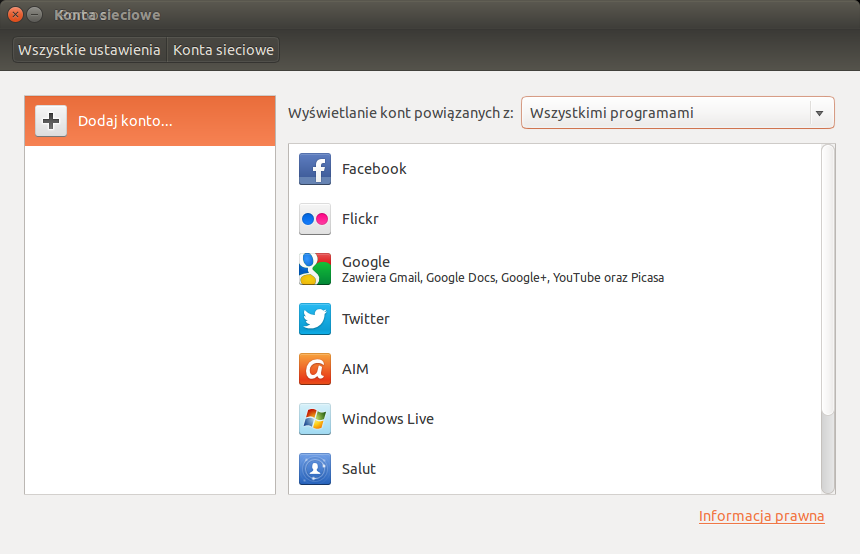
\includegraphics[width=\linewidth]{images/programy_kontaOnline1.png}
\end{center}

Aby dodać konto do systemu wyszukaj w Dashu \textcolor{ubuntu_orange}{Konta Sieciowe} i uruchom program. W otwartym oknie kliknij \textcolor{ubuntu_orange}{+ Dodaj konto} w lewym panelu a następnie a prawego panelu wybierz interesującego cię dostawcę. Zostaniesz teraz poproszony o uwierzytelnienie usługi w systemie.

Możesz zsynchronizować więcej niż jedną usługę. Ponadto program Konta Sieciowe pozwala zarządzać które programy mają dostęp do których usług. 